\section{Feature Engineering}

Most of the score jump came from feature work, not from swapping one model for another. The raw columns were already useful, but they hid the borrower story. We got much better results once we started writing features that sounded like lending questions instead of spreadsheet formulas.

\begin{table}[H]
    \centering
    \small
    \begin{tabularx}{\linewidth}{@{} p{0.22\linewidth} p{0.34\linewidth} X @{}}
        \toprule
        Feature family & Examples & Why it stayed in the final public pipeline \\
        \midrule
        Affordability ratios & loan share of income, monthly payment share, asset coverage & These features turned raw balances into simple stress indicators and helped both targets. \\
        Delinquency features & weighted late-payment counts, severity over history length, utilization interactions & They were consistently strong for \texttt{RiskTier} and also improved rate prediction. \\
        Derogatory burden & charge-off, collection, bankruptcy, and public-record aggregates & A compact way to summarize past damage without relying on a single raw field. \\
        Semantic missingness & renter-without-property, owner-without-mortgage, no-collateral flags & These features captured why a field was blank, which was often more useful than the filled value itself. \\
        Controlled interactions & selected pairwise products between stress and balance features & A small interaction set helped the tree models find sharper non-linear boundaries. \\
        \bottomrule
    \end{tabularx}
    \caption{Feature groups that mattered enough to survive into the best public lane.}
    \label{tab:feature-families}
\end{table}

Figure~\ref{fig:feature-signal} shows the same pattern from another angle. The two targets overlap, but they do not rank features in exactly the same way. Delinquency and utilization features dominate the classification side, while affordability and balance-sheet coverage matter a bit more for the rate regression.

\begin{figure}[H]
    \centering
    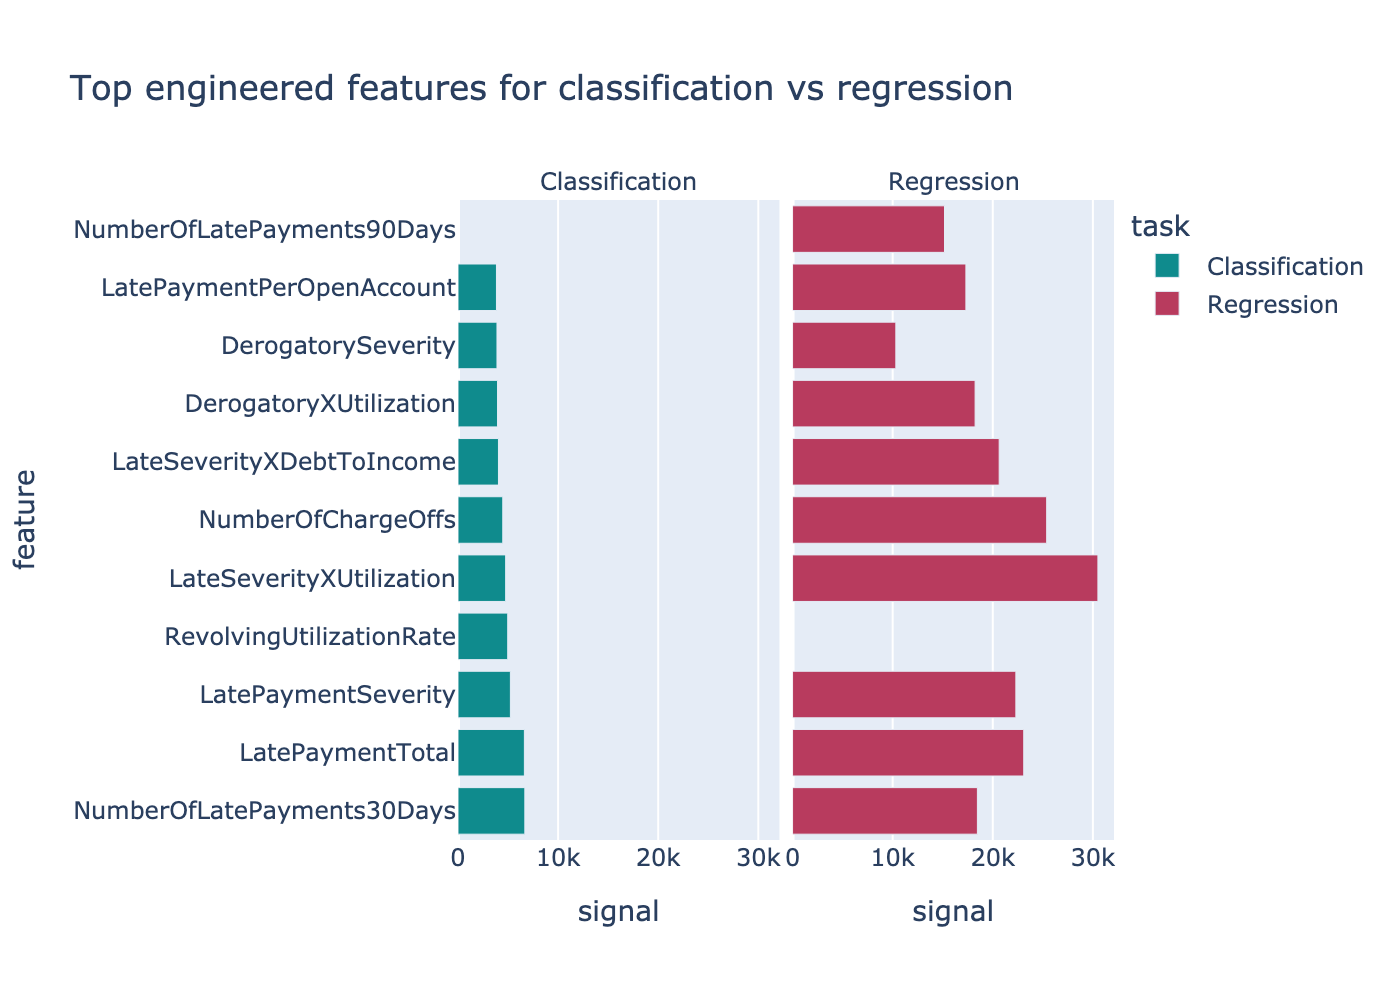
\includegraphics[width=\linewidth]{figures/feature_signal_comparison.png}
    \caption{The strongest engineered features overlap across targets, but the ordering is not identical.}
    \label{fig:feature-signal}
\end{figure}

We also tracked how the score changed when major feature ideas were added. The important pattern is not that every extra trick helped, but that the first few feature families changed the game while later additions gave smaller and more selective gains. The overall project progression later in the report follows the same logic.
